\documentclass{book}

%Post to: https://stats.stackexchange.com/questions/21346/reference-book-for-linear-algebra-applied-to-statistics

\usepackage[top=1in, bottom=1.25in, left=1.25in, right=1.25in]{geometry}

\usepackage{amsfonts, amsmath}
\usepackage{commath}
\usepackage[yyyymmdd,hhmmss]{datetime}
\usepackage{graphbox}
\usepackage[hidelinks]{hyperref}
\usepackage{marginnote}
\usepackage{mathtools}
\usepackage{parskip}
\usepackage{titlesec}
\usepackage{xcolor}
\usepackage{optidef}

\usepackage{makeidx}
\makeindex

\usepackage[numbers,sort&compress]{natbib}
\bibliographystyle{unsrtnat}

%Make equations be numbered continuously through book
\usepackage{chngcntr}
\counterwithout{equation}{chapter}

\renewcommand*{\pd}[3][]{\ensuremath{\frac{\partial^{#1} #2}{\partial #3}}}

\newcommand{\mA}{\mathbf{A}}
\newcommand{\mB}{\mathbf{B}}
\newcommand{\mC}{\mathbf{C}}
\newcommand{\mD}{\mathbf{D}}
\newcommand{\mF}{\mathbf{F}}
\newcommand{\mH}{\mathbf{H}}
\newcommand{\mI}{\mathbf{I}}
\newcommand{\mJ}{\mathbf{J}}
\newcommand{\mL}{\mathbf{L}}
\newcommand{\mM}{\mathbf{M}}
\newcommand{\mP}{\mathbf{P}}
\newcommand{\mQ}{\mathbf{Q}}
\newcommand{\mR}{\mathbf{R}}
\newcommand{\mU}{\mathbf{U}}
\newcommand{\mV}{\mathbf{V}}
\newcommand{\mX}{\mathbf{X}}
\newcommand{\mY}{\mathbf{Y}}
\newcommand{\va}{\mathbf{a}}
\newcommand{\vb}{\mathbf{b}}
\newcommand{\vc}{\mathbf{c}}
\newcommand{\vd}{\mathbf{d}}
\newcommand{\vg}{\mathbf{g}}
\newcommand{\vp}{\mathbf{p}}
\newcommand{\vq}{\mathbf{q}}
\newcommand{\vu}{\mathbf{u}}
\newcommand{\vv}{\mathbf{v}}
\newcommand{\vw}{\mathbf{w}}
\newcommand{\vx}{\mathbf{x}}
\newcommand{\vy}{\mathbf{y}}
\newcommand{\vz}{\mathbf{z}}
\DeclareMathOperator{\diag}{diag}
\DeclareMathOperator{\eig}{eig}
\DeclareMathOperator{\trace}{tr}
\DeclareMathOperator{\rank}{rank}
\newcommand{\sPSD}{\mathbb{S}^n_+}
\newcommand{\sC}{\mathbb{C}}
\newcommand{\sCmn}{\mathbb{C}^{m,n}}
\newcommand{\sCnn}{\mathbb{C}^{n,n}}
\newcommand{\sR}{\mathbb{R}}
\newcommand{\sRm}{\mathbb{R}^{m}}
\newcommand{\sRn}{\mathbb{R}^{n}}
\newcommand{\sRp}{\mathbb{R}^{p}}
\newcommand{\sRnm}{\mathbb{R}^{n,m}}
\newcommand{\sRmn}{\mathbb{R}^{m,n}}
\newcommand{\sRnn}{\mathbb{R}^{n,n}}
\newcommand{\sRnp}{\mathbb{R}^{n,p}}
\newcommand{\sRnr}{\mathbb{R}^{n,r}}
\newcommand{\sRmm}{\mathbb{R}^{m,m}}
\newcommand{\sSn}{\mathbb{S}^{n}}
\newcommand{\ispsd}{\succeq}
\newcommand{\ispd}{\succ}
\newcommand{\pinv}{\!^+}
\newcommand{\ns}{\mathcal{N}}
\newcommand{\range}{\mathcal{R}}
\newcommand{\bs}{\setminus}

\hypersetup{
  pdfauthor={Richard Barnes (ORCID: 0000-0002-0204-6040)},%
  pdftitle={Matrix Forensics},%
%            pdfsubject={Whatever},%
  pdfkeywords = {matrix algebra, matrix relations, matrix identities, linear algebra},%
  pdfproducer = {LaTeX},%
  pdfcreator  = {pdfLaTeX}
}


\usepackage{fancyhdr}
% \renewcommand{\chaptermark}[1]{\markboth{#1}{#1}}
\setlength{\headheight}{15.2pt}
\pagestyle{fancy}

\lhead[\thepage]{\leftmark}
% \chead[]{<odd output>}
\rhead[\leftmark]{\thepage}

\renewcommand{\footrulewidth}{0.4pt}% default is 0pt
\lfoot[\footnotesize{Richard Barnes. Matrix Forensics. \today-\currenttime. \href{https://github.com/r-barnes/MatrixForensics}{github.com/r-barnes/MatrixForensics}}. \input{/tmp/matrix_forensics_version.info}\!\!.]{\footnotesize{Richard Barnes. Matrix Forensics. \today-\currenttime. \href{https://github.com/r-barnes/MatrixForensics}{github.com/r-barnes/MatrixForensics}}. \input{/tmp/matrix_forensics_version.info}\!\!.} %  [<even output>]{<odd output>}
\cfoot[]{}
\rfoot[]{}


\newcommand{\eqcite}[1]{\marginnote{\citep{#1}}}

%Adjust chapter formatting
\newcommand{\hsp}{\hspace{20pt}}
\definecolor{gray75}{gray}{0.75}
\titleformat{\chapter}[hang]{\Huge\bfseries}{\thechapter\hsp\textcolor{gray75}{$|$}\hsp}{0pt}{\Huge\bfseries}
\titlespacing*{\chapter}{0pt}{0pt}{20pt} %? BEFORE AFTER

%Ensure chapters start on the same page
\usepackage{etoolbox}
\makeatletter
\patchcmd{\chapter}{\if@openright\cleardoublepage\else\clearpage\fi}{\clearpage}{}{}
\makeatother


\begin{document}

\begin{titlepage} % Suppresses displaying the page number on the title page and the subsequent page counts as page 1
  \raggedleft % Right align the title page
  
  \rule{1pt}{\textheight} % Vertical line
  \hspace{0.05\textwidth} % Whitespace between the vertical line and title page text
  \parbox[b]{0.75\textwidth}{ % Paragraph box for holding the title page text, adjust the width to move the title page left or right on the page
    
    {\Huge\bfseries Matrix Forensics \\[\baselineskip]} % Title
    {\large\textit{A brief guide to matrix math \\ and its efficient implementation}}\\[4\baselineskip] % Subtitle or further description
    {\Large\textsc{richard barnes}} % Author name, lower case for consistent small caps
    \\[4\baselineskip]
    \href{https://github.com/r-barnes/MatrixForensics}{github.com/r-barnes/MatrixForensics}
    
    \vspace{0.6\textheight} % Whitespace between the title block and the publisher
    
    %{\noindent The Publisher~~\plogo}\\[\baselineskip] % Publisher and logo
  }

\end{titlepage}


\tableofcontents

\chapter{Introduction}

\textbf{Goals:}
\begin{enumerate}
\item The primary goal of \textit{Matrix Forensics} is to \textbf{solve crimes of matrix math}.
That is, to make the sometimes mystifying manipulations of matrix math more understandable by cataloging useful identities, transformations, and facts.

\item \textbf{To be a community-accessible project.} Anyone can contribute to the project. The source code for the book is available on Github and the source code has been thoughtfully arranged with handy macros to help maintain an easy-to-use, aesthetic, and consistent notation and typography.
\end{enumerate}


\textbf{Contributing:}
Please contribute on Github at \url{https://github.com/r-barnes/MatrixForensics} either by opening an issue or making a pull request. If you are not comfortable with this, please send your contribution to \url{rijard.barnes@gmail.com}.


\textbf{Contributors:}
Richard Barnes

\textbf{Funding:}

The Department of Energy Computational Science Graduate Fellowship (grant DE-FG02-97ER25308). %Richard Barnes

\chapter{Nomenclature}

\begin{tabular}{cl}
$\mA$                   & Matrix.                                                   \\
$\va$                   & (Column) vector.                                          \\
$a$                     & Scalar.                                                   \\
$\lambda$               & An eigenvalue of a matrix.                                \\
& \\
$\mA_{ij}$              & Matrix indexed. Returns $i$th row and $j$th column.       \\
$\mA\circ \mB$          & Hadamard (element-wise) product of matrices A and B.      \\
$\ns(\mA)$              & Nullspace of the matrix $\mA$.                            \\
$\range(\mA)$           & Range of the matrix $\mA$.                                \\
$\det(\mA)$             & Determinant of the matrix $\mA$.                          \\
$\eig(\mA)$             & Eigenvalues of the matrix $\mA$.                          \\
$\mA^H$                 & Conjugate transpose of the matrix $\mA$.                  \\
$\mA^T$                 & Transpose of the matrix $\mA$.                            \\
$\mA\pinv$              & Pseudoinverse of the matrix $\mA$.                        \\
$\vx\in\sRn$            & The entries of the $n$-vector $\vx$ are all real numbers. \\
$\mA\in\sRmn$           & The entries of the matrix $\mA$ with $m$ rows and $n$ columns are all real numbers. \\
$\mA\in\sSn$            & The matrix $\mA$ is symmetric and has $n$ rows and $n$ columns. \\
& \\
$\mI_n$                 & Identity matrix with $n$ rows and $n$ columns.            \\
& \\
$\{0\}$                 & The empty set       \\
$\sR$                   & The real numbers    \\
$\sC$                   & The complex numbers
\end{tabular}

\chapter{Basics}

\section{Fundamental Theorem of Linear Algebra}

\begin{center}
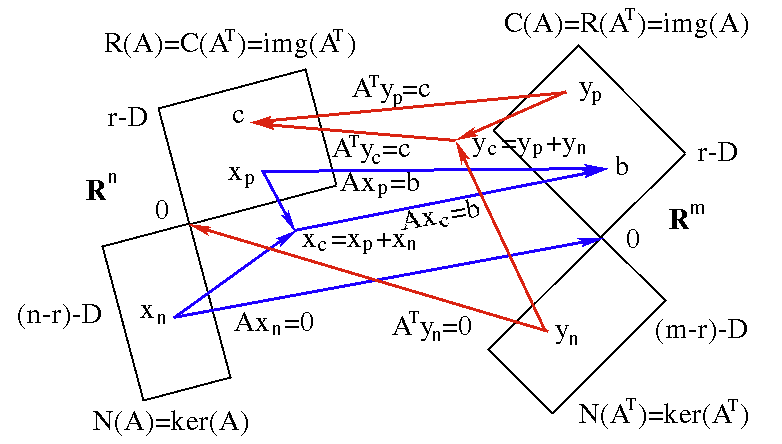
\includegraphics[width=\textwidth]{imgs/fund_theorem_lin_alg1.png}
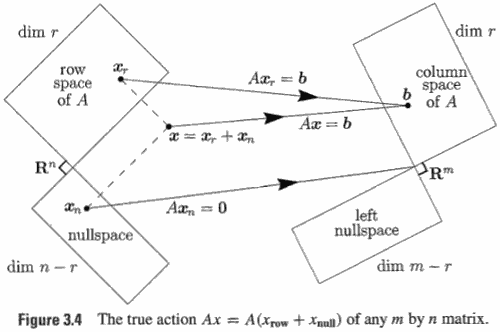
\includegraphics[width=\textwidth]{imgs/fund_theorem_lin_alg2.png}
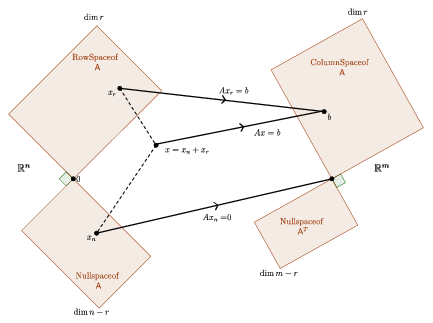
\includegraphics[width=\textwidth]{imgs/fund_theorem_lin_alg3.png}
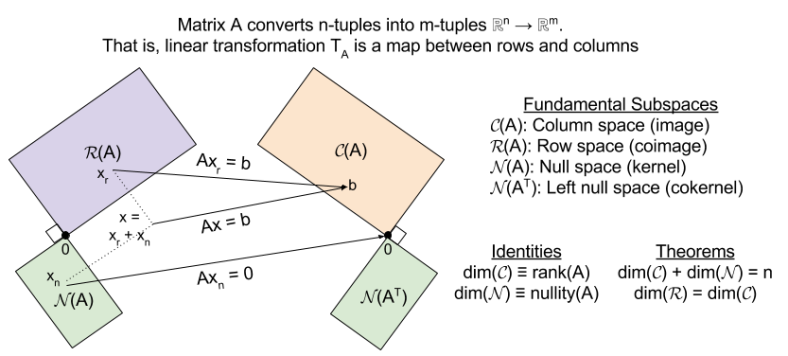
\includegraphics[width=\textwidth]{imgs/fund_theorem_lin_alg4.png}
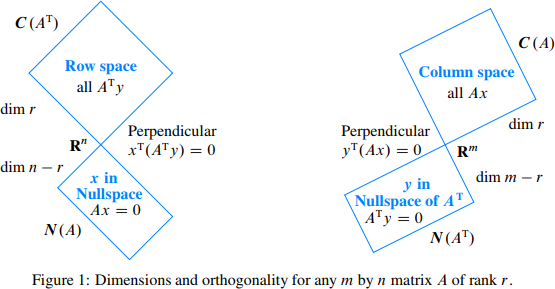
\includegraphics[width=\textwidth]{imgs/fund_theorem_lin_alg5.png}
\end{center}


\section{Matrix Properties}

\begin{align}
\mA(\mB+\mC) &=   \mA\mB+\mA\mC &\textrm{(left distributivity)}   \\
(\mB+\mC)\mA &=   \mB\mA+\mC\mA &\textrm{(right distributivity)}  \\
\mA\mB       &\ne \mB\mA        &\textrm{(in general)}            \\
(\mA\mB)\mC  &=   \mA(\mB\mC)   &\textrm{(associativity)}
\end{align}

\section{Rank}

\begin{align}
\noalign{If $\mA\in\sRmn$ and $\mB\in\sRnr$, then}
\eqcite{Thome2016}
\rank(\mA)+\rank(\mB)-n\le \rank(\mA\mB)\le \min(\rank(\mA),\rank(\mB)) &&~~~~\textrm{Sylvester's Inequality} \\
\noalign{If $\mA\mB$, $\mA\mB\mC$, $\mB\mC$ are defined, then}
\eqcite{Thome2016}
\rank(\mA\mB)+\rank(\mB\mC)\le \rank(\mB)+\rank(\mA\mB\mC) && \textrm{Frobenius's inequality} \\
\noalign{If $\dim(\mA)=\dim(\mB)$, then}
\rank(\mA+\mB)\le\rank(\mA)+\rank(\mB) &&\textrm{Subadditivity}
\end{align}
If $\mA_1, \mA_2, \ldots, \mA_l$ have $n_1,n_2,\ldots,n_l$ columns, so that $\mA_1\mA_2\ldots\mA_l$ is well-defined, then
\begin{equation}
\eqcite{Thome2016}
\rank(\mA_1\mA_2\ldots\mA_l)
\ge \sum_{i=1}^{l-1}\rank(\mA_i\mA_{i+1})-\sum_{i=2}^{l-1}\rank(\mA_i)
\ge\sum_{i=1}^l\rank(\mA_i)-\sum_{i=1}^{l-1}n_i 
\end{equation}

\section{Identities}
\begin{align}
\left(\sum_{i=1}^n \vz_i\right)^2 = \vz^T
\begin{bmatrix}
1      & \hdots & 1      \\
\vdots & \ddots & \vdots \\
1      & \hdots & 1      
\end{bmatrix}
\vz
\end{align}

\section{Matrix Multiplication}

For $\mA\in\sR^{i,j}$ and $\mB\in\sR^{j,k}$ and $\mC\in\sR^{l,k}$
\begin{align}
[\mA\mB]_{ik} &= \sum_j \mA_{ij}\mB_{jk} \\
[\mA\mB\mC^T]_{il} &= \sum_j \mA_{ij}[\mB\mC^T]_{jl}=\sum_j \mA_{ij}\sum_k \mB_{jk}\mC_{lk}=\sum_j\sum_k \mA_{ij}\mB_{jk}\mC_{lk}
\end{align}



\section{Time Complexities}
\begin{center}
{\footnotesize\renewcommand{\arraystretch}{1.2}
\begin{tabular}{p{1.5cm}p{3cm}p{3cm}p{4cm}p{1cm}}
\textbf{Operation}             & \textbf{Input}                   & \textbf{Output}    & \textbf{Algorithm}                     & \textbf{Time}   \\ \hline
Matmult
    & $A,B\in n\times n$
    & $n \times n$
    & Schoolbook
    & $O(n^3)$
    \\ \hline

    &
    &
    & Strassen~\citep{Strassen1969}
    & $O(n^{2.807})$
    \\ \hline

    &
    &
    & Best
    & $O(n^\omega)$
    \\ \hline
Matmult
    & $A\in n\times m, B\in m\times p$
    & $n \times p$
    & Schoolbook
    & $O(nmp)$
    \\ \hline
Inversion
    & $A\in n\times n$
    & $n \times n$
    & Gauss--Jordan elimination
    & $O(n^3)$
    \\ \hline

    &
    &
    & Strassen~\citep{Strassen1969}
    & $O(n^{2.807})$
    \\ \hline

    &
    &
    & Best
    & $O(n^\omega)$
    \\ \hline
SVD
    & $A\in m\times n$
    & $m\times m, m\times n, n\times n$ \newline $m\times r, r\times r, n\times r$
    &
    & $O(mn^2)$ \newline \hbox{$(m\ge n)$} \\ \hline
Determinant
    & $A\in n\times n$
    & Scalar
    & Laplace expansion
    & $O(n!)$         \\ \hline

    &
    &
    & Division-free~\citep{Rote2001}
    & $O(n!)$
    \\ \hline

    &
    &
    & LU decomposition
    & $O(n^3)$
    \\ \hline

    &
    &
    & Integer preserving~\citep{Bareiss1968}
    & $O(n^3)$
    \\ \hline
Back \newline substitution
    & $A$ triangular
    & $n$ solutions
    & Back substitution
    & $O(n^2)$
    \\ \hline
\end{tabular}
}
\end{center}

\subsubsection{A comment on $\omega$}

The lower bound on matmult time complexity is $O(n^\omega)$, where $\omega$ is an unknown constant bounded by $2\le\omega\le2.373$. Algorithms achieving lower values of $\omega$ tend to be less efficient in practice for all but the largest matrices. Of the algorithm with times of less than $O(n^3)$, only the Strassen algorithm has seen serious attempts at optimized implementation. Most matmult implementations use highly optimized variants of the standard $O(n^3)$ algorithm. At this point, memory and bus speeds dominate the performance of implementations, so simple Big-O notation cannot be used to reliably compare matmult performances.

\begin{center}
\begin{tabular}{lll}
\textbf{Name}           & \textbf{Year} & $\omega$  \\
Standard                & -             & 3         \\
\citet{Strassen1969}    & 1969          & 2.807     \\
\citet{Pan1978}         & 1978          & 2.796     \\
\citet{Bini1979}        & 1979          & 2.78      \\
\citet{Schonhage1981}   & 1981          & 2.548     \\
\citet{Schonhage1981}   & 1981          & 2.522     \\
\citet{Romani1982}      & 1982          & 2.517     \\
\citet{Coppersmith1982} & 1982          & 2.496     \\
\citet{Strassen1986}    & 1986          & 2.479     \\
\citet{Copper1990}      & 1990          & 2.376     \\
\citet{Williams2012}    & 2012          & 2.37294   \\
\citet{LeGall2014}      & 2014          & 2.3728639 \\
\citet{Williams2012}    & 2012          & 2.3727    \\
\end{tabular}
\end{center}

%TODO: Include handy diagram from https://explained.ai/matrix-calculus/index.html

\chapter{Derivatives}

\section{Useful Rules for Derivatives}
For general $\mA$ and $\mX$ (no special structure):
\begin{align}
\partial\mA           &= 0~~\textrm{where $\mA$ is a constant} \\
\partial(c\mX)        &= c\partial\mX                          \\
\partial(\mX+\mY)     &= \partial\mX+\partial\mY               \\
\partial(\trace(\mX)) &= \trace(\partial(\mX))                 \\
\partial(\mX\mY)      &= (\partial\mX)\mY + \mX(\partial\mY)   \\
\partial(\mX\circ\mY) &= (\partial\mX)\circ\mY + \mX\circ(\partial\mY) \\
%TODO Kronecker x in circle equation 39 Matrix Cookbook
\partial(\mX^{-1})    &= -\mX^{-1}(\partial\mX)\mX^{-1}        \\
\partial(\det(\mX))   &= \trace(\textrm{adj}(\mX)\partial\mX)  \\
\partial(\det(\mX))   &= \det(\mX)\trace(\mX^{-1}\partial\mX)  \\
\partial(\ln(\det(\mX))) &= \trace(\mX^{-1}\partial\mX)        \\
\partial(\mX^T)       &= (\partial\mX)^T                       \\
\partial(\mX^H)       &= (\partial\mX)^H
\end{align}

\section{Gradient Notation}
For a matrix $\mA\in\sRnm$, the gradient is defined as:
\begin{equation}
\grad_\mA f(\mA)=
\begin{bmatrix}
\pd{f(\mA)}{\mA_{11}} & \pd{f(\mA)}{\mA_{12}} & \ldots & \pd{f(\mA)}{\mA_{1n}} \\
\pd{f(\mA)}{\mA_{21}} & \pd{f(\mA)}{\mA_{22}} & \ldots & \pd{f(\mA)}{\mA_{2n}} \\
\vdots                & \vdots                & \ddots & \vdots                \\
\pd{f(\mA)}{\mA_{m1}} & \pd{f(\mA)}{\mA_{m2}} & \ldots & \pd{f(\mA)}{\mA_{mn}}
\end{bmatrix}
\end{equation}
i.e.
\begin{equation}
(\grad_\mA f(\mA))_{ij}=\pd{f(\mA)}{\mA_{ij}}
\end{equation}
Note that the size of the gradient is always the same size as the entity to which it is taken. Also note that the gradient of a function is only defined if the function is real-valued, that is, if it returns a scalar value.

\section{Derivatives of Matrices and Vectors}

\subsection{First-Order}

In the following, $\mJ$ is the Single-Entry Matrix (\autoref{sec:rogue_single_entry}).
\begin{align}
\pd{\vx^T \va}{\vx}     &= \pd{\va^T \vx}{\vx} = \va          \\
\pd{\va^T\mX\vb}{\mX}   &= \va\vb^T                           \\
\pd{\va^T\mX^T\vb}{\mX} &= \vb\va^T                           \\
\pd{\va^T\mX\va}{\mX}   &= \pd{\va^T\mX^T\va}{\mX} = \va\va^T \\
\pd{\mX}{\mX_{ij}}      &= \mJ^{ij}                              %TODO: What is this? (MCB 73)
%TODO: MCB 74, 75
\end{align}

\section{Derivatives of vector norms}

\begin{align}
\pd{}{\vx}\norm{\vx-\va}_2 &= \frac{\vx-\va}{\norm{\vx-\va}_2} \\
\pd{}{\vx}\frac{\vx-\va}{\norm{\vx-\va}_2} &= \frac{\mI}{\norm{\vx-\va}_2}-\frac{(\vx-\va)(\vx-\va)^T}{\norm{\vx-\va}_2^3} \\
\pd{\norm{\vx}_2^2}{\vx} &= \pd{\norm{\vx^T\vx}_2}{\vx} = 2\vx
\end{align}

\section{Scalar by Vector}
\begin{center}
\begin{tabular}{l|Sc|Sc|Sc}
Qualifier                  & Expression                                    & Numerator layout                                   & Denominator layout                            \\
                           & $\pd{a}{x}$                                   & $\vzero^T$                                         & $\vzero$                                      \\
                           & $\pd{au(\vx)}{\vx}$                           & $a\pd{u}{\vx}$                                     & Same                                          \\
                           & $\pd{u(\vx)+v(\vx)}{\vx}$                     & $\pd{u}{\vx} + \pd{v}{\vx}$                        & Same                                          \\
                           & $\pd{u(\vx)v(\vx)}{\vx}$                      & $u\pd{v}{\vx} + v\pd{u}{\vx}$                      & Same                                          \\
                           & $\pd{g(u(\vx))}{\vx}$                         & $\pd{g(u)}{u}\pd{u}{\vx}$                          & Same                                          \\
                           & $\pd{f(g(u(\vx)))}{\vx}$                      & $\pd{f(g)}{g}\pd{g(u)}{u}\pd{u}{\vx}$              & Same                                          \\
                           & $\pd{\vu(\vx)^T\vv(\vx)}{\vx}$                & $\vu^T\pd{\vv}{\vx}+\vv^T\pd{\vu}{\vx}$            & $\pd{\vu}{\vx}\vv+\pd{\vv}{\vx}\vu$           \\
                           & $\pd{\vu(\vx)^T\mA\vv(\vx)}{\vx}$             & $\vu^T\mA\pd{\vv}{\vx}+\vv^T\mA^T\pd{\vu}{\vx}$    & $\pd{\vu}{\vx}\mA\vv+\pd{\vv}{\vx}\mA^T\vu$   \\
                           & $\md{f}{2}{\vx}{}{{\vx^T}}{}$                 &                                                    & $\mH$, the Hessian matrix                     \\
                           & $\pd{\va\cdot\vx}{\vx}=\pd{\vx\cdot\va}{\vx}$ & $\va^T$                                            & $\va$                                         \\
                           & $\pd{\vb^T\mA\vx}{\vx}$                       & $\vb^T\mA$                                         & $\mA^T\vb$                                    \\
                           & $\pd{\vx^T\mA\vx}{\vx}$                       & $\vx^T(\mA+\mA^T)$                                 & $(\mA+\mA^T)\vx$                              \\
$\mA$ symmetric            & $\pd{\vx^T\mA\vx}{\vx}$                       & $2\vx^T\mA$                                        & $2\mA\vx$                                     \\
                           & $\pd{\vx^T\mA\vx}{\vx}$                       & $\mA+\mA^T$                                        & Same                                          \\
$\mA$ symmetric            & $\pd{\vx^T\mA\vx}{\vx}$                       & $\mA$                                              & Same                                          \\
                           & $\pd{\vx^T\vx}{\vx}$                          & $2\vx^T$                                           & $2\vx$                                        \\
                           & $\pd{\va^T\vu(\vx)}{\vx}$                     & $\va^T\pd{\vu}{\vx}$                               & $\pd{\vu}{\vx}\va$                            \\
                           & $\pd{\va^T\vx\vx^T\vb}{\vx}$                  & $\vx^T(\va\vb^T+\vb\va^T)$                         & $(\va\vb^T+\vb\va^T)\vx$                      \\
                           & $\pd{(\mA\vx+\vb)^T\mC(\mD\vx+\ve)}{\vx}$     & $(\mD\vx+\ve)^T\mC^T\mA+(\mA\vx+\vb)^T\mC\mD$      & $\mD^T\mC^T(\mA\vx+\vb)+\mA^T\mC(\mD\vx+\ve)$ \\
                           & $\pd{\norm{\vx-\va}}{\vx}$                    & $\frac{(\vx-\va)^T}{\norm{\vx-\va}}$               & $\frac{\vx-\va}{\norm{\vx-\va}}$              \\                           
\end{tabular}
\end{center}

\section{Vector by Vector}
\begin{center}
\begin{tabular}{l|Sc|Sc|Sc}
Qualifier                  & Expression                                    & Numerator layout                                   & Denominator layout                            \\
                           & $\pd{\va}{\vx}$                               & $\vzero$                                           & Same                                          \\ %TODO: really the same? shouldn't be transposed?
                           & $\pd{\vx}{\vx}$                               & $\mI$                                              & Same                                          \\ %TODO: Really the identity matrix? Which one?
                           & $\pd{\mA\vx}{\vx}$                            & $\mA$                                              & $\mA^T$                                       \\
                           & $\pd{\vx^T\mA}{\vx}$                          & $\mA^T$                                            & $\mA$                                         \\
                           & $\pd{a\vu(\vx)}{\vx}$                         & $a\pd{\vu}{\vx}$                                   & Same                                          \\
                           & $\pd{a(\vx)\vu(\vx)}{\vx}$                    & $a\pd{\vu}{\vx}+\vu\pd{a}{\vx}$                    & $a\pd{\vu}{\vx}+\pd{a}{\vx}\vu^T$             \\
                           & $\pd{\mA\vu(\vx)}{\vx}$                       & $\mA\pd{\vu}{\vx}$                                 & $\pd{\vu}{\vx}\mA^T$                          \\
                           & $\pd{(\vu(\vx)+\vv(\vx))}{\vx}$               & $\pd{\vu}{\vx}+\pd{\vv}{\vx}$                      & Same                                          \\
                           & $\pd{\vg(\vu(\vx))}{\vx}$                     & $\pd{\vg(\vu)}{\vu}\pd{\vu}{\vx}$                  & $\pd{\vu}{\vx}\pd{\vg(\vu)}{\vu}$             \\
                           & $\pd{\vf(\vg(\vu(\vx)))}{\vx}$                & $\pd{\vf(\vg)}{\vg(\vu)}\pd{\vg(\vu)}{\vu}\pd{\vu}{\vx}$& $\pd{\vu}{\vx}\pd{\vg(\vu)}{\vu}\pd{\vf(\vg)}{\vg}$
\end{tabular}
\end{center}



\section{Matrix by Scalar}
\begin{center}
\begin{tabular}{l|Sc|Sc}
Qualifier                  & Expression                                     & Numerator layout                                       \\
                           & $\pd{a\mU(x)}{x}$                              & $a\pd{\mU}{x}$                                         \\
                           & $\pd{\mA\mU(x)\mB}{x}$                         & $\mA\pd{\mU}{x}\mB$                                    \\
                           & $\pd{(\mU(x)+\mV(x))}{x}$                      & $\pd{\mU}{x}+\pd{\mV}{x}$                              \\
                           & $\pd{(\mU(x)\mV(x))}{x}$                       & $\mU\pd{\mV}{x}+\pd{\mU}{x}\mV$                        \\
                           & $\pd{(\mU(x)\kp\mV(x))}{x}$                    & $\mU\kp\pd{\mV}{x} + \pd{\mU}{x}\kp\mV$                \\
                           & $\pd{(\mU(x)\hp\mV(x))}{x}$                    & $\mU\hp\pd{\mV}{x} + \pd{\mU}{x}\hp\mV$                \\
                           & $\pd{\mU^{-1}(x)}{x}$                          & $-\mU^{-1} \pd{\mU}{x} \mU^{-1}$                       \\
                           & $\md{\mU^{-1}}{2}{x}{}{y}{}$                   & $\mU^{-1}\left(\pd{\mU}{x}\mU^{-1}\pd{\mU}{y} - \md{\mU}{2}{x}{}{y}{} + \pd{\mU}{y}\mU^{-1}\pd{\mU}{x}\right)\mU^{-1}$ \\
                           & $\pd{e^{x\mA}}{x}$                             & $\mA e^{x\mA}=e^{x\mA}\mA$
\end{tabular}
\end{center}

\chapter{Matrix Rogue Gallery}

\section{Non-Singular vs.\ Singular Matrices}
For $\mA\in\sRnn$ (initially drawn from \citep[p.\ 574]{Strang2016}):
\begin{center}
\begin{tabular}{ll}
\textbf{Non-Singular}                           & \textbf{Singular}                        \\
$\mA$ is invertible                             & $\mA$ is not invertible                  \\
The columns are independent                     & The columns are dependent                \\
The rows are independent                        & The rows are dependent                   \\
$\det(\mA)\ne0$                                 & $\det(\mA)=0$                            \\
$\mA\vx=0$ has one solution: $\vx=0$            & $\mA\vx=0$ has infinitely many solutions \\
$\mA\vx=\vb$ has one solution: $\vx=\mA^{-1}\vb$& $\mA\vx=\vb$ has either no or infinitely many solutions \\
$\mA$ has $n$ nonzero pivots                    & $\mA$ has $r<n$ pivots                   \\
$\mA$ has full rank $r=n$                       & $\mA$ has rank $r<n$                     \\
The reduced row echelon form is $\mR=\mI$       & $\mR$ has at least one zero row          \\
The column space is all of $\sRn$               & The column space has dimension $r<n$     \\
The row space is all of $\sRn$                  & The row space has dimension $r<n$        \\
All eigenvalues are nonzero                     & Zero is an eigenvalue of $\mA$           \\
$\mA^T\mA$ is symmetric positive definite       & $\mA^T\mA$ is only semidefinite          \\
$\mA$ has $n$ positive singular values          & $\mA$ has $r<n$ singular values        
\end{tabular}
\end{center}

\section{Diagonal Matrix}

\begin{center}
\includegraphics[width=1.5in]{imgs/rg_diagonal.pdf}
\end{center}

\begin{equation}
A=\diag(a_1,\ldots,a_n)=
\begin{bmatrix}
a_1  &        &  \\
     & \ddots &  \\
     &        & a_n 
\end{bmatrix}
\end{equation}

Square matrix. Entries above diagonal are equal to entries below diagonal.

Number of ``free entries": $\frac{n(n+1)}{2}$.

\subsection*{Special Properties}

\begin{equation}
\eig(A)={a_1,\ldots,a_n}
\end{equation}

\begin{equation}
\det(A)=\prod_i a_i 
\end{equation}

\begin{equation}
A^{-1}=
\begin{bmatrix}
\frac{1}{a_1} &        &               \\
              & \ddots &               \\
              &        & \frac{1}{a_n}
\end{bmatrix}
\end{equation}




\section{Dyads}

\begin{center}
\includegraphics[width=2in]{imgs/rg_dyad.pdf}
\end{center}

$\mA\in\sRmn$ is a dyad if it can be written as
\begin{equation}
\mA=\vu\vv^T~~~\vu\in\sRm, \vv\in\sRn
\end{equation}

\subsection*{Special Properties}
\begin{itemize}
\item The columns of $\mA$ are copies of $\vu$ scaled by the values of $\vv$.
\item The rows of $\mA$ are copies of $\vu^T$ scaled by the values of $\vv$.
\item If $\mA$ is a dyad, it acts on a vector $\vx$ as $\mA\vx=(\vu\vv^T)\vx=(\vv^T\vu)\vx$.
\item $\mA\vx=c\vu$ ($\mA$ scales $\vx$ and points it along $\vu$).
\item $\mA_{ij}=\vu_i\vv_j$.
\item If $\vu,\vv\ne0$, then $\rank(\mA)=1$.
\item If $m=n$, $\mA$ has one eigenvalue $\lambda=\vv^T\vu$ and eigenvector $\vu$.
\item A dyad can always be written in a normalized form $c\tilde\vu\tilde\vv^T$.
\end{itemize}



\section{Hermitian Matrix}
$\mH\in\sCmn$ is Hermitian iff
\begin{equation}
\mH=\mH^H
\end{equation}
where $\mH^H$ is the conjugate transpose of $\mH$.

For $\mH\in\sRmn$, Hermitian and symmetric matrices are equivalent.

\subsection*{Special Properties}
\begin{align}
\mH_{ii} &\in \sR      \\
\mH\mH^H &=   \mH^H\mH \\
\vx^H\mH\vx &\in \sR~~\forall\vx\in\sC \\
\mH_1+\mH_2 &= \textrm{Hermitian} \\
\mH^{-1}    &= \textrm{Hermitian} \\
\mA+\mA^H   &= \textrm{Hermitian} \\
\mA-\mA^H   &= \textrm{Skew-Hermitian} \\
\mA\mB      &= \textrm{Hermitian iff $\mA\mB=\mB\mA$} \\
\det(\mH)   &\in \sR \\
\eig(\mH)   &\in \sR
\end{align}



\section{Idempotent Matrix}
A matrix $\mA$ is idempotent iff
\begin{equation}
\mA\mA=\mA
\end{equation}

\subsection*{Special Properties}
\begin{align}
\mA^n        &=A~~\forall n              \\
\mI-\mA      &~~\textrm{is idempotent}   \\
\mA^H        &~~\textrm{is idempotent}   \\
\mI-\mA^H    &~~\textrm{is idempotent}   \\
\rank(\mA)   &= \trace(\mA)              \\
\mA(I-\mA)   &= 0                        \\
\mA\pinv     &= \mA                      \\
f(s\mI+t\mA) &= (\mI-\mA)f(s)+\mA f(s+t) \\
\mA\mB=\mB\mA&\implies \mA\mB~\textrm{is idempotent} \\
\eig(\mA)_i  &\in \{0,1\} \\
\mA & \textrm{~is always diagonalizable}
\end{align}
$\mA-\mI$ may not be idempotent.




\section{Orthogonal Matrix}

\begin{center}
\includegraphics[width=1.5in]{imgs/rg_orthogonal.pdf}

(Not much visible structure)
\end{center}


\begin{equation}
U=
\begin{bmatrix}
1 & 0 & 0 & 0 & 0 & 0 \\
0 & 0 & 0 & 0 & 1 & 0 \\
0 & 0 & 1 & 0 & 0 & 0 \\
0 & 1 & 0 & 0 & 0 & 0 \\
0 & 0 & 0 & 0 & 0 & 1 \\
0 & 0 & 0 & 1 & 0 & 0 \\
\end{bmatrix}
\end{equation}

A matrix $\mU$ is orthogonal iff:

\begin{equation}
\mU^T \mU = \mU \mU^T = I
\end{equation}

Square matrix. The columns form an orthonormal basis of $\mathbb{R}^n$.



\subsection*{Special Properties}

\begin{itemize}
\item The eigenvalues of $\mU$ are placed on the unit circle.
\item The eigenvectors of $\mU$ are unitary (have length one).
\item $\mU^{-1}$ is orthogonal.
\end{itemize}

\begin{align}
\mU^T     &= \mU^{-1} \\
\mU^{-T}  &= \mU      \\
\mU^T\mU  &= \mI      \\
\mU\mU^T  &= \mI      \\
\det(\mU) &= \pm1
\end{align}



Orthogonal matrices preserve the lengths and angles of the vectors they operator on. The converse is true: any matrix which preserves lengths and angles is orthogonal.
\begin{equation}
\norm{\mU \vx}^2_2=(\mU\vx)^T(\mU\vx)=\vx^T\mU^T\mU\vx=\vx^T\vx=\norm{\vx}^2_2~~\forall \vx
\end{equation}
\begin{equation}
\norm{\mU \mA \mV}_F=\norm{\mA}_F~~\forall \mA,\mU,\mV~\textrm{with}~\mU,\mV \textrm{orthogonal}
\end{equation}



\section{Permutation Matrix}
\begin{center}
\includegraphics[width=1.5in]{imgs/rg_permutation_matrix.pdf}
\end{center}

TODO



\section{Positive Definite}

$\mA\in\sSn$ is positive definite (denoted $\mA\ispd0$) if any of the following are true:
\begin{itemize}
\item $\vx^T\mA\vx>0,\forall\vx\in\sRn$.
\item $\eig(\mA)>0$
\end{itemize}


\subsection*{Special Properties}

\begin{itemize}
\item If $\mA$ is PD and invertible, $\mA^{-1}$ is also PD.
\item If $\mA$ is PD and $c\in\sR$ then $c\mA$ is PD.
\item The diagonal entries $\mA_{ii}$ are real and non-negative, so $\trace(\mA)\ge0$. %TODO: Shouldn't this be >0?
\item $\det(\mA)>0$
\item For $\mA\in\sRmn$, $\mA^T\mA\ispd0\iff \mA$ is full-column rank ($\rank(\mA)=n$)
\item For $\mA\in\sRmn$, $\mA\mA^T\ispd0\iff \mA$ is full-row rank ($\rank(\mA)=m$)
\item $\mP\ispd0$ defines a full-dimensional, bounded ellipsoid centered at the origin and defined by the set $\mathcal{E}=\{\vx\in\sRn: x^T\mP^{-1}x\le1\}$. The eigenvalues $\lambda_i$ and eigenvectors $u_i$ of $\mP$ define the orientation and shape of the ellipsoid. $u_i$ are the semi-axes while the lengths of the semi-axes are given by $\sqrt{\lambda_i}$. Using the Cholesky decomposition, $\mP^{-1}=\mA^T\mA$, an equivalent definition of the ellipsoid is $\mathcal{E}=\{\vx\in\sRn: \norm{\mA\vx}_2\le1\}$.
\end{itemize}

\section{Positive Semi-Definite}

$\mA$ is positive semi-definite (denoted $\mA\ispsd0$) if any of the following are true:
\begin{itemize}
\item $\vx^T\mA\vx\ge0,\forall\vx\in\sRn$.
\item $\eig(\mA)\ge0$
\end{itemize}

\subsection*{Special Properties}
\begin{itemize}
\item For $\mA\in\sRmn$, $\mA^T\mA\ispsd0$
\item For $\mA\in\sRmn$, $\mA\mA^T\ispsd0$
\item The positive semi-definite matrices $\sPSD$ form a convex cone. For any two PSD matrices $\mA,\mB\in\sPSD$ and some $\alpha\in[0,1]$:
\begin{equation}
\vx^T(\alpha\mA+(1-\alpha)\mB)\vx=\alpha \vx^T\mA\vx+(1-\alpha)\vx^T\mB\vx\ge0~~\forall\vx
\end{equation}
\begin{equation}
\alpha\mA+(1-\alpha)\mB\in\sPSD
\end{equation}
\item For $\mA\in\sPSD$ and $\alpha\ge0$, $\alpha\mA\ispsd0$, so $\sPSD$ is a cone.
\end{itemize}

\subsection{Loewner order}
If $\mA-\mB\ispsd 0$, then we say $\mA\ispsd \mB$. A sufficient condition for this is that $\lambda_n(\mA)\ge\lambda_1(\mB)$.



\section{Projection Matrix}
A square matrix $\mP$ is a projection matrix that projects onto a vector space $\mathcal{S}$ iff
\begin{align}
\mP&~\textrm{is idempotent} \\
\mP\vx&\in\mathcal{S}~~\forall\vx \\
\mP\vz&=\vz~~\forall\vz\in\mathcal{S}
\end{align}


\section{Single-Entry Matrix}
\label{sec:rogue_single_entry} 
\begin{equation}
\mJ^{2,3} =
\begin{bmatrix}
0 & 0 & 0 & 0 \\
0 & 0 & 1 & 0 \\
0 & 0 & 0 & 0 \\
0 & 0 & 0 & 0
\end{bmatrix}
\end{equation}

The single-entry matrix $\mJ^{iJ}\in\sRnn$ is defined as the matrix which is zero everywhere except for the entry $(i,j)$, which is $1$.


%TODO: Much material from MCB



\section{Singular Matrix}
A square matrix that is not invertible.

$\mA\in\sRnn$ is singular iff $\det \mA=0$ iff $\mathcal{N}(A)\ne\{0\}$.


\section{Symmetric Matrix}

\begin{center}
\includegraphics[width=1.5in]{imgs/rg_symmetric_matrix.pdf}
\end{center}

$\mA\in\sSn$ is a symmetric matrix if $\mA=\mA^T$ (entries above diagonal are equal to entries below diagonal).

\begin{equation}
\begin{bmatrix}
a & b & c & d & e & f \\
b & g & l & m & o & p \\
c & l & h & n & q & r \\
d & m & n & i & s & t \\
e & o & q & s & j & u \\
f & p & r & t & u & k \\
\end{bmatrix}
\end{equation}


\subsection*{Special Properties}

\begin{align}
\mA                                &=   \mA^T \\
\eig(A)                            &\in \sRn  \\
\textrm{Number of ``free entries"} &=    \frac{n(n+1)}{2}
\end{align}

If $\mA$ is real, it can be decomposed into $\mA=\mQ^T\mD\mQ$ where $\mQ$ is a real orthogonal matrix (the columns of which are eigenvectors of $\mA$) and $\mD$ is real and diagonal containing the eigenvalues of $\mA$.

For a real, symmetric matrix with non-negative eignevalues, the eigenvalues and singular values coincide.



\section{Skew-Hermitian}
A matrix $\mH\in\sCmn$ is Skew-Hermitian iff
\begin{equation}
\mH=-\mH^H
\end{equation}



\section{Toeplitz Matrix, General Form}

\begin{center}
\includegraphics[width=1.5in]{imgs/rg_toeplitz.pdf}
\end{center}
Constant values on descending diagonals.
\begin{equation}
\begin{bmatrix}
  a_{0} & a_{-1} & a_{-2} & \ldots  & \ldots & a_{-(n-1)}  \\
  a_{1} & a_0    & a_{-1} & \ddots  &        & \vdots \\
  a_{2} & a_{1}  & \ddots & \ddots  & \ddots & \vdots \\ 
 \vdots & \ddots & \ddots & \ddots  & a_{-1} & a_{-2}\\
 \vdots &        & \ddots & a_{1}   & a_{0}  & a_{-1} \\
a_{n-1} & \ldots & \ldots & a_{2}   & a_{1}  & a_{0}
\end{bmatrix}
\end{equation}


\section{Toeplitz Matrix, Discrete Convolution}

\begin{center}
\includegraphics[width=1.5in]{imgs/rg_toeplitz_1d_conv.pdf}
\end{center}

Constant values on main and subdiagonals.

\begin{equation}
\begin{bmatrix}
  h_m &   0 &   0 &      \hdots &   0 &   0 \\
  \vdots & h_m &   0 &   \hdots &   0 &   0 \\
  h_1 & \vdots & h_m &   \hdots &   0 &   0 \\
    0 & h_1 & \ddots & \ddots &   0 &   0 \\
    0 &   0 & h_1 &    \ddots & h_m &   0 \\
    0 &   0 &   0 &    \ddots & \vdots & h_m \\
    0 &   0 &   0 &      \hdots & h_1 & \vdots \\
    0 &   0 &   0 &      \hdots &   0 & h_1 
\end{bmatrix}
\end{equation}


\section{Triangular Matrix}

\begin{center}
\includegraphics[width=1.5in]{imgs/rg_lower_triangular.pdf}~\includegraphics[width=1.5in]{imgs/rg_upper_triangular.pdf}
\end{center}

\begin{equation}
\begin{bmatrix}
a & b & c & d & e & f \\
  & g & h & i & j & k \\
  &   & l & m & n & o \\
  &   &   & p & q & r \\
  &   &   &   & s & t \\
  &   &   &   &   & u \\
\end{bmatrix}
~
~
\begin{bmatrix}
a &   &   &   &   &   \\
b & g &   &   &   &   \\
c & h & l &   &   &   \\
d & i & m & p &   &   \\
e & j & n & q & s &   \\
f & k & o & r & t & u \\
\end{bmatrix}
\end{equation}

Square matrices in which all elements either above or below the main diagonal are zero. An upper (left) and a lower (right) triangular matrix are shown above.

For an upper triangular matrix $A_{ij}=0$ whenever $i>j$; for a lower triangular matrix $A_{ij}=0$ whenever $i<j$.


\subsection*{Special Properties}

\begin{align}
\eig(A) &= \diag(A)             \\
\det(A) &= \prod_i \diag(A)_i
\end{align}

The product of two upper (lower) triangular matrices is still upper (lower) triangular.

The inverse of a nonsingular upper (lower) triangular matrix is still upper (lower) triangular.




\section{Vandermonde Matrix}
\begin{equation}
V=
\begin{bmatrix}
1      & \alpha_1 & \alpha_1^2 & \dots  & \alpha_1^{n-1} \\
1      & \alpha_2 & \alpha_2^2 & \dots  & \alpha_2^{n-1} \\
1      & \alpha_3 & \alpha_3^2 & \dots  & \alpha_3^{n-1} \\
\vdots & \vdots   & \vdots     & \ddots & \vdots         \\
1      & \alpha_m & \alpha_m^2 & \dots  & \alpha_m^{n-1}
\end{bmatrix}
\end{equation}
Alternatively,
\begin{equation}
V_{i,j} = \alpha_i^{j-1}
\end{equation}

\subsection*{Uses}
Polynomial interpolation of data.

\subsection*{Special Properties}
\begin{itemize}
\item $\det(V)=\prod_{1\le i < j \le n} (x_j-x_i)$
\end{itemize}

\chapter{Matrix Decompositions}

\section{LLT/UTU: Cholesky Decomposition} %TODO: Add UU to TOC

\begin{center}
\includegraphics[align=c,height=1in]{imgs/decomp_cholesky_a.pdf}\textbf{\large =}
\includegraphics[align=c,height=1in]{imgs/decomp_cholesky_L.pdf}\textbf{\large *}
\includegraphics[align=c,height=1in]{imgs/decomp_cholesky_LT.pdf}
\end{center}

If $\mA$ is symmetric, positive definite, square, then
\begin{equation}
\mA=\mU^T\mU=\mL\mL^T
\end{equation}
where $\mU$ is a unique upper triangular matrix and $\mL$ is a unique lower-triangular matrix.

\section{LDLT}

\begin{center}
\includegraphics[align=c,height=1in]{imgs/decomp_ldlt_a.pdf}\textbf{\large =}
\includegraphics[align=c,height=1in]{imgs/decomp_ldlt_L.pdf}\textbf{\large *}
\includegraphics[align=c,height=1in]{imgs/decomp_ldlt_D.pdf}\textbf{\large *}
\includegraphics[align=c,height=1in]{imgs/decomp_ldlt_LT.pdf}
\end{center}

If $\mA$ is a non-singular symmetric definite square matrix, then
\begin{equation}
\mA=\mL\mD\mL^T=\mL^T\mD\mL
\end{equation}
where $\mL$ is a unit lower triangular matrix and $\mD$ is a diagonal matrix. If $\mA\ispd0$, then $\mD_{ii}>0$.

% For $\mA\in\sRnn$,
% \begin{align}
% \mA&\ispsd0\iff \exists\mB\ispsd0: \mA=\mB^2 \\
% \mA&\ispd0 \iff \exists\mB\ispd 0: \mA=\mB^2
% \end{align}
% where $\mB$ is called the ``matrix square-root" of $\mA$.

% For $\mA\ispsd0$, we can use the spectral factorization $\mA=\mU\mD\mU^T$ and take $\mD^{1/2}=\diag(\sqrt{\lambda_1},\ldots,\sqrt{\lambda_n})$ to get $\mB=\mU\mD^{1/2}\mU^T$.


\section{PCA: Principle Components Analysis}
Find normalized directions in data space such that the variance of the projections of the centered data points is maximal. For centered data $\tilde \mX$, the mean-square variation of data along a vector $\vx$ is $\vx^T \tilde \mX \tilde \mX^T \vx$.
\begin{equation}
\max_{\vx\in\sRn,~\norm{\vx}_2=1} \vx^T \tilde \mX \tilde \mX^T \vx
\end{equation}
Taking an SVD of $\tilde \mX \tilde \mX^T$ gives $H=\mU_r\mD^2\mU^T$, which is maximized by taking $\vx=\vu_1$. By repeatedly removing the first principal components and recalculating, all the principal axes can be found.




\section{QR: Orthogonal-triangular}

\begin{center}
\includegraphics[align=c,height=1in]{imgs/decomp_qr_a.pdf}\textbf{\large =}
\includegraphics[align=c,height=1in]{imgs/decomp_qr_q.pdf}\textbf{\large *}
\includegraphics[align=c,height=1in]{imgs/decomp_qr_r.pdf}
\end{center}

For $\mA\in\sRnn$, $\mA=\mQ\mR$ where $\mQ$ is orthogonal and $\mR$ is an upper triangular matrix. If $\mA$ is non-singular, then $\mQ$ and $\mR$ are uniquely defined if $\diag(\mR)$ are imposed to be positive.

\subsection*{Algorithms}

Gram-Schmidt.




\section{SVD: Singular Value Decomposition}

\begin{center}
\includegraphics[align=c,height=1in]{imgs/decomp_svd_a.pdf}\textbf{\large =}
\includegraphics[align=c,height=1in]{imgs/decomp_svd_u.pdf}\textbf{\large *}
\includegraphics[align=c,height=1in]{imgs/decomp_svd_s.pdf}\textbf{\large *}
\includegraphics[align=c,height=1in]{imgs/decomp_svd_v.pdf}
\end{center}

\begin{center}
\includegraphics[align=c,width=0.5in]{imgs/decomp_svd_a_compact.pdf}\textbf{\large =}
\includegraphics[align=c,width=0.5in]{imgs/decomp_svd_u_compact.pdf}\textbf{\large *}
\includegraphics[align=c,width=0.5in]{imgs/decomp_svd_s_compact.pdf}\textbf{\large *}
\includegraphics[align=c,width=0.5in]{imgs/decomp_svd_v_compact.pdf}
\end{center}

Any matrix $\mA\in\sRmn$ can be written as
\begin{equation}
\mA=\mU \mD \mV^T=\sum_{i=1}^r \sigma_i u_i v_i^T
\end{equation}
where
\begin{align}
U&=\textrm{eigenvectors of~}\mA\mA^T & \sRmm \\
D&=\diag(\sigma_i)=\sqrt{\diag(\eig(\mA\mA^T))}      & \sRnm \\
V&=\textrm{eigenvectors of~}\mA^T\mA & \sRnn
\end{align}
Let $\sigma_i$ be the non-zero singular values for $i=1,\ldots,r$ where $r$ is the rank of $\mA$; $\sigma_1\ge\ldots\ge\sigma_r$.

We also have that
\begin{align}
\mA   \vv_i &= \sigma_i \vu_i \\
\mA^T \vu_i &= \sigma_i \vv_i \\
\mU^T\mU &= \mI \\
\mV^T\mV &= \mI
\end{align}

$\mD$ can be written in an expanded form:
\begin{equation}
\tilde \mD=
\begin{bmatrix}
\mD       & 0_{r,n-r}   \\
0_{m-r,r} & 0_{m-r,n-r}
\end{bmatrix}
\end{equation}
The final $n-r$ columns of $\mV$ give an orthonormal basis spanning $\ns(\mA)$. An orthonormal basis spanning the range of $\mA$ is given by the first $r$ columns of $\mU$.

\begin{align}
\norm{\mA}^2_F&=\textrm{Frobenius norm} =\trace(\mA^T\mA)=\sum_{i=1}^r \sigma_i^2 \\
\norm{\mA}^2_2&=\sigma_1^2 \\
\norm{\mA}_* &= \textrm{nuclear norm}=\sum_{i=1}^r \sigma_i
\end{align}

The \textbf{condition number} $\kappa$ of an invertible matrix $\mA\in\sRnn$ is the ratio of the largest and smallest singular value. Matrices with large condition numbers are closer to being singular and more sensitive to changes.
\begin{equation}
\kappa(\mA)=\frac{\sigma_1}{\sigma_n}=\norm{A}_2 \cdot \norm{A^{-1}}_2
\end{equation}

\subsection*{Low-Rank Approximation}
Approximating $\mA\in\sRmn$ by a matrix $\mA_k$ of rank $k>0$ can be formulated as the optimization probem
\begin{equation}
\min_{\mA_k\in\sRmn} \norm{\mA-\mA_k}_F^2: \rank{\mA_k}=k, 1\le k \le \rank(\mA)
\end{equation}
The optimal solution of this problem is given by
\begin{equation}
\mA_k=\sum_{i=1}^k \sigma_i \vu_i \vv_i^T
\end{equation}
where
\begin{align}
\frac{\norm{\mA_k}_F^2}{\norm{\mA}_F^2}&=\frac{\sigma_1^2+\ldots+\sigma_k^2}{\sigma_1^2+\ldots+\sigma_r^2} \\
1-\frac{\norm{\mA_k}_F^2}{\norm{\mA}_F^2}&=\frac{\sigma_{k+1}^2+\ldots+\sigma_r^2}{\sigma_1^2+\ldots+\sigma_r^2} 
\end{align}
is the fraction of the total variance in $\mA$ explained by the approximation $\mA_k$.

\subsection*{Range and Nullspace}
\begin{align}
\ns(\mA) &= \range(\mV_{nr})                      \\
\ns(\mA)^\perp \equiv\range(\mA^T)&=\range(\mV_r) \\
\range(\mA)&=\range(\mU_r)                        \\
\range(\mA)^\perp\equiv\ns(\mA^T)&=\range(\mU_{nr})
\end{align}
where $\mV_r$ is the first $r$ columns of $V$ and $V_nr$ are the last $[r+1,n]$ columns; similarly for $\mU$.


\subsection*{Projectors}
The projection of $\vx$ onto $\ns(\mA)$ is $(\mV_{nr}\mV_{nr}^T)\vx$. Since $\mI_n=\mV_r\mV_r^T+\mV_{nr}\mV_{nr}^T$, $(\mI_n-\mV_{r}\mV_{r}^T)\vx$ also works. The projection of $\vx$ onto $\range(\mA)$ is $(\mU_r\mU_r^T)\vx$.

If $\mA\in\sRmn$ is full row rank ($\mA\mA^T\ispd0$), then the minimum distance to an affine set $\{x:\mA\vx=\vb\}, \vb\in\sRm$ is given by $\vx^*=\mA^T(\mA\mA^T)^{-1}\vb$. %TODO

If $\mA\in\sRmn$ is full column rank ($\mA^T\mA\ispd0$), then the minimum distance to an affine set $\{x:\mA\vx=\vb\}, \vb\in\sRm$ is given by $\vx^*=\mA(\mA^T\mA)^{-1}\mA^T\vb$. %TODO


\subsection*{Computational Notes}
A \textit{numerical rank} can be estimated for the matrix as the largest $k$ such that $\sigma_k>\epsilon \sigma_1$ for $\epsilon\ge0$.



\section{Eigenvalue Decomposition for Diagonalizable Matrices}

For a square, diagonalizable matrix $\mA\in\mathbb{R}^{n,n}$ 
\begin{equation}
\mA=U\Lambda U^{-1}
\end{equation}
where $U\in\mathbb{C}^{n,n}$ is an invertible matrix whose columns are the eigenvectors of $\mA$ and $\Lambda$ is a diagonal matrix containing the eigenvalues $\lambda_1,\ldots,\lambda_n$ of $\mA$ in the diagonal.

The columns $\vu_1,\ldots,\vu_n$ satisfy
\begin{equation}
\mA \vu_i=\lambda_i \vu_i~~i=1,\ldots,n
\end{equation}

\section{Eigenvalue (Spectral) Decomposition for Symmetric Matrices}

A symmetric matrix $\mA\in\mathbb{R}^{n,n}$ can be factored as
\begin{equation}
\mA=U\Lambda U^T=\sum_i^n \lambda_i \vu_i \vu_i^T
\end{equation}
where $U\in\mathbb{R}^{n,n}$ is an orthogonal matrix whose columns $\vu_i$ are the eigenvectors of $\mA$ and $\Lambda$ is a diagonal matrix containing the eigenvalues $\lambda_1\ge\ldots\ge\lambda_n$ of $\mA$ in the diagonal. These eigenvalues are always real. The eigenvectors can always be chosen to be real and to form an orthonormal basis.

The columns $\vu_1,\ldots,\vu_n$ satisfy
\begin{equation}
\mA \vu_i=\lambda_i \vu_i~~i=1,\ldots,n
\end{equation}


\section{Schur Complements}

For $\mA\in\sSn$, $\mB\in\sSn$, $\mX\in\sRnm$ with $\mB\ispd0$ and the block matrix
\begin{equation}
\mM=
\begin{bmatrix}
\mA & \mX \\
\mX^T & \mB
\end{bmatrix}
\end{equation}
and the Schur complement of $\mA$ in $\mM$
\begin{equation}
S=\mA-\mX\mB^{-1}\mX^T
\end{equation}
Then
\begin{align}
\mM\ispsd0&\iff S\ispsd0 \\
\mM\ispd0 &\iff S\ispd0 
\end{align}





\chapter{Transpose Properties}

\begin{align}
(\mA\mB)^T   &= \mB^T\mA^T    \\
(\mA+\mB)^T  &= \mA^T+\mB^T   \\
(\mA^{-1})^T &= (\mA^T)^{-1}
\end{align}


\chapter{Determinant Properties}

Geometrically, if a unit volume is acted on by $\mA$, then $|\det(\mA)|$ indicates the volume after the transformation.
\begin{align}
\det(I_n)          &= 1                                   \\
\det(\mA^T)        &= \det(\mA)                           \\
\det(\mA^{-1})     &= \frac{1}{\det(\mA)}=\det(\mA)^{-1}  \\
\det(\mA\mB)       &= \det(\mB\mA)                        \\
\det(\mA\mB)       &= \det(\mA)\det(\mB)                  &\mA,\mB\in\sRnn \\
\det(c\mA)         &= c^n\det(\mA)                        &\mA\in\sRnn     \\
\det(\mA)          &= \prod \eig(\mA)                     \\
\noalign{For $\mA\in\sRmn, \mB\in\sRnm$}
\eqcite{Sylvester1851}
\det(\mI_m+\mA\mB) &= \det(\mI_n+\mB\mA) & & \textrm{Sylvester's determinant identity}
\end{align}


\chapter{Trace Properties}
\begin{align}
\trace(\mA)    &=\sum_{i=1}^n \mA_{ii}   & \mA\in\sRnn \\
\trace(\mA+\mB)&=\trace(\mA)+\trace(\mB) \\
\trace(c\mA)   &=c\trace(\mA)            \\
\trace(\mA)    &=\trace(\mA^T)
\end{align}

For $\mA,\mB,\mC,\mD$ of compatible dimensions,

\begin{equation}
\trace(\mA^T\mB)=\trace(\mA\mB^T)=\trace(\mB^T\mA)=\trace(\mB\mA^T)
\end{equation}
\begin{equation}
\trace(\mA\mB\mC\mD)=\trace(\mB\mC\mD\mA)=\trace(\mC\mD\mA\mB)=\trace(\mD\mA\mB\mC)
\end{equation}
(Invariant under cyclic permutations)



\chapter{Inverse Properties}
The inverse of $\mA\in\sCnn$ is denoted $\mA^{-1}$ and defined such that
\begin{equation}
\mA\mA^{-1}=\mA^{-1}\mA=\mI_n
\end{equation}
where $\mI_n$ is the $n \times n$ identity matrix. $\mA$ is nonsingular if $\mA^{-1}$ exists; otherwise, $\mA$ is singular.


If individual inverses exist
\begin{equation}
(\mA\mB)^{-1}=\mB^{-1}\mA^{-1}
\end{equation}
more generally
\begin{equation}
(\mA_1\mA_2\ldots\mA_n)^{-1}=\mA_n^{-1}\ldots\mA_2^{-1}\mA_1^{-1}
\end{equation}

\begin{equation}
(\mA^{-1})^T=(\mA^T)^{-1}
\end{equation}




\chapter{Pseudo-Inverse Properties}
For $\mA\in\sRmn$, a pseudoinverse satisfies:
\begin{align}
\mA\mA\pinv\mA      &= \mA         \\
\mA\pinv\mA\mA\pinv &= \mA\pinv    \\
(\mA\mA\pinv)^T     &= \mA\mA\pinv \\
(\mA\pinv\mA)^T     &= \mA\pinv\mA
\end{align}

\section{Moore-Penrose Pseudoinverse}
\begin{equation}
\mA\pinv = \mV \mD^{-1} \mU^T
\end{equation}
where the foregoing comes from a singular-value decomposition and $\mD^{-1}=\diag(\frac{1}{\sigma_1},\ldots,\frac{1}{\sigma_r})$

\subsection*{Special Properties}
\begin{itemize}
\item $\mA\pinv=\mA^{-1}$ if $\mA\in\sRnn$ and $\mA$ is square and nonsingular.
\item $\mA\pinv=(\mA^T\mA)^{-1}\mA^T$, if $\mA\in\sRmn$ is full column rank ($r=n\le m$). $\mA\pinv$ is a left inverse of $\mA$, so $\mA\pinv\mA=\mV_r\mV_r^T=\mV\mV^T=\mI_n$.
\item $\mA\pinv=\mA^T(\mA\mA^T)^{-1}$, if $\mA\in\sRmn$ is full row rank ($r=m\le n$). $\mA\pinv$ is a right inverse of $\mA$, so $\mA\mA\pinv=\mU_r\mU_r^T=\mU\mU^T=\mI_m$.
\end{itemize} %TODO: Check these



\chapter{Hadamard Identities}

\begin{align}
(\mA\circ\mB)_{ij}    &= A_{ij}B_{ij}~\forall~i,j                                     \\
\mA\circ\mB           &= \mB\circ\mA                             \eqcite{million2007} \\
\mA\circ(\mB\circ\mC) &= (\mA\circ\mB)\circ\mC                                        \\
\mA\circ(\mB+\mC)     &= \mA\circ\mB+\mA\circ\mC                 \eqcite{million2007} \\
a(\mA\circ\mB)        &= (a\mA)\circ\mB =\mA\circ(a\mB)          \eqcite{million2007} \\
(\mA^T\circ\mB^T)     &= (\mA\circ\mB)^T                                              \\
(\mA^T\circ\mB^T)     &= (\mA\circ\mB)^T                                              \\
(\vx^T \mA \vx)       &= \sum_{i,j}\big((\vx \vx^T)\circ\mA\big)                      \\
\vx^T(\mA\circ\mB)\vy &= \trace((\diag(\vx)\mA)^T \mB\diag(\vy))~~~\mA,\mB\in\sRmn \eqcite{Minka2000}   \\
\trace(\mA^T\mB)      &= \mathbf{1}^T(\mA\circ\mB)\mathbf{1}                          
\end{align}


\chapter{Eigenvalue Properties}

$\lambda\in\mathbb{C}$ is an eigenvalue of $\mA\in\sRnn$ and $u\in\mathbb{C}^n$ is a corresponding eigenvector if $\mA\vu=\lambda\vu$ and $\vu\ne0$. Equivalantly, $(\lambda \mI_n-\mA)\vu=0$ and $\vu\ne0$. Eigenvalues satisfy the equation $\det(\lambda\mI_n-\mA)=0$.

Any matrix $\mA\in\sRnn$ has $n$ eigenvalues, though some may be repeated. $\lambda_1$ is the largest eigenvalue and $\lambda_n$ the smallest.

\begin{equation}
\eig(\mA\mA^T)=\eig(\mA^T\mA)
\end{equation}
(Note that the number of entries in $\mA\mA^T$ and $\mA^T\mA$ may differ significantly leading to different compute times.)

\begin{equation}
\eig(\mA^T\mA)\ge0
\end{equation}

\begin{equation}
\lambda_\textrm{min}(\mA)\le \frac{\vx^T \mA \vx}{\vx^T\vx} \le \lambda_\textrm{max}(\mA)~~\vx\ne0
\end{equation}

\subsection{Weyl's Inequality}
If $\mM,\mH,\mP\in\sRnn$ are Hermitian matrices and $\mM=\mH+\mP$ ($\mH$ is perturbed by $\mP$) and $\mM$ has eigenvalues $\mu_1\ge\cdots\ge\mu_n$, $\mH$ has eigenvalues $\nu_1\ge\cdots\ge\nu_n$, and $\mP$ has eigenvalues $\rho_1\ge\cdots\ge\rho_n$, then
\begin{equation}
\nu_i+\rho_n\le \mu_i \le \nu_i + \rho_1~\forall i
\end{equation}
If $j+k-n\ge i \ge r+s-1$, then
\begin{equation}
\nu_j+\rho_k\le\mu_i\le\nu_r+\rho_s
\end{equation}
If $\mP\ispsd0$, then $\mu_i>\nu_i~\forall i$.

%TODO
% \section*{Computation}
% TODO: eigsh, small eigen value extraction, top-k







\chapter{Norms}

\section{General Properties}
Matrix norms satisfy some properties:
\begin{align}
f(\mA)    &\ge 0             \\
f(\mA)    &=   0  \iff \mA=0 \\
f(c\mA)   &=   |c|f(\mA)     \\
f(\mA+\mB)&\le f(\mA)+f(\mB)
\end{align}
Many popular norms also satisfy ``sub-multiplicativity": $f(\mA\mB)\le f(\mA)f(\mB)$.

\section{Matrices}

\subsection{Frobenius norm}
\begin{align}
\norm{\mA}_F &= \sqrt{\trace\mA\mA^H}                           \\
             &= \sqrt{\sum_{i=1}^m \sum_{j=1}^n |\mA_{ij}|^2 }  \\
             &= \sqrt{\sum_{i=1}^m \eig(A^H A)_i }
\end{align}

\subsubsection{Special Properties}
\begin{align}
\norm{\mA\vx}_2         &\le \norm{\mA}_F \norm{\vx}_2~~~\vx\in\sRn \\
\norm{\mA\mB}_F         &\le \norm{\mA}_F \norm{\mB}_F \\
\norm{\mC-\vx\vx^T}_F^2 &= \norm{\mC}_F^2+\norm{\vx}_2^4-2 \vx^T \mC \vx
\end{align}

\subsection{Operator Norms}
For $p=1,2,\infty$ or other values, an operator norm indicates the maximum input-output gain of the matrix.
\begin{equation}
\norm{\mA}_p=\max_{\norm{\vu}_p=1} \norm{\mA\vu}_p
\end{equation}

\begin{align}
\norm{\mA}_1
  &=\max_{\norm{\vu}_1=1} \norm{\mA\vu}_1       \\
  &=\max_{j=1,\ldots,n} \sum_{i=1}^m |\mA_{ij}| \\
  &=\textrm{Largest absolute column sum}
\end{align}

\begin{align}
\norm{\mA}_\infty
  &=\max_{\norm{\vu}_\infty=1} \norm{\mA\vu}_\infty  \\
  &=\max_{j=1,\ldots,m} \sum_{i=1}^n |\mA_{ij}| \\
  &=\textrm{Largest absolute row sum}
\end{align}

\begin{align}
\norm{\mA}_2
  &=\textrm{``spectral norm"}                   \\
  &=\max_{\norm{\vu}_2=1} \norm{\mA\vu}_2       \\
  &=\sqrt{\max(\eig(\mA^T\mA))} \\
  &=\textrm{Square root of largest eigenvalue of~}\mA^T\mA
\end{align}



\subsubsection{Special Properties}
\begin{align}
\norm{\mA\vu}_p &\le \norm{\mA}_p \norm{\vu}_p \\
\norm{\mA\mB}_p &\le \norm{\mA}_p \norm{\mB}_p 
\end{align}

\subsection{Spectral Radius}
Not a proper norm.
\begin{equation}
\rho(\mA)=\textrm{spectral radius}(\mA)=\max_{i=1,\ldots,n} | \eig(\mA)_i |
\end{equation}

\subsubsection{Special Properties}
\begin{align}
\rho(\mA) &\le \norm{\mA}_p \\
\rho(\mA) &\le \min(~\norm{\mA}_1, \norm{\mA}_\infty)
\end{align}


\section{Vectors}

\begin{align}
\norm{\vx}_1      &= \sum_i |\vx_i|           & \textrm{L1-norm\index{L1-norm}} \\
\norm{\vx}_p      &= (\sum_i |\vx_i|^p)^{1/p} & \textrm{P-norm\index{P-norm}}   \\
\norm{\vx}_\infty &= \max_i |\vx_i|           & \textrm{L$\infty$-norm\index{L$\infty$-norm}, L-infinity norm}
\end{align}

\subsection{Identities}

\begin{align}
2\norm{\vu}_2^2+2\norm{\vv}_2^2 &= \norm{\vu+\vv}_2^2 + \norm{\vu-\vv}_2^2                                                      & \textrm{Polarization Identity} \\
<\vx,\vy>                       &= \frac{1}{4}\left(\norm{\vx+\vy}_2^2-\norm{\vx-\vy}_2^2\right)~~\forall \vx,\vy\in\mathcal{V} & \textrm{Polarization Identity} \\
\norm{u}_2^2+\norm{v}_2^2&=\norm{\begin{bmatrix} u \\ v\end{bmatrix}}_2^2
\end{align}


\subsection{Bounds}

\begin{align}
|\vx^T \vy| &\le \norm{\vx}_2 \norm{\vy}_2 & \textrm{Cauchy-Schwartz Inequality} \\
|\vx^T \vy| &\le \sum_{k=1}^n |\vx_k \vy_k| \le \norm{\vx}_p \norm{\vx}_q~~~\forall p,q\ge1: 1/p+1/q=1 & \textrm{H\"older Inequality}
\end{align}

For $\vx\in\mathbb{R}^n$
\begin{equation}
\frac{1}{\sqrt{n}}\norm{\vx}_2
\le\norm{\vx}_\infty
\le\norm{\vx}_2
\le\norm{\vx}_1
\le\sqrt{\textrm{card}(\vx)}\norm{\vx}_2
\le\sqrt{n}\norm{\vx}_2
\le n \norm{\vx}_\infty
\end{equation}

For any $0<p<q$ we have that $\norm{\vx}_q\le\norm{\vx}_p$.



\chapter{Bounds} %TODO: Reorganize

\section{Matrix Gain}
\begin{equation}
\lambda_\textrm{min}(\mA^T\mA)\le \frac{\norm{\mA\vx}_2^2}{\norm{\vx}_2^2}\le\lambda_\textrm{max}(\mA^T\mA)
\end{equation}

\begin{equation}
\max_{\vx\ne0} \frac{\norm{\mA\vx}_2}{\norm{\vx}_2}=\norm{\mA}_2=\sqrt{\lambda_\textrm{max}(\mA^T\mA)}\implies\vx=u_1
\end{equation}

\begin{equation}
\min_{\vx\ne0} \frac{\norm{\mA\vx}_2}{\norm{\vx}_2}=\sqrt{\lambda_\textrm{min}(\mA^T\mA)}\implies\vx=u_n
\end{equation}

\section{Rayleigh quotients}
The Rayleigh quotient of $\mA\in\sSn$ is given by
\begin{equation}
\frac{\vx^T \mA \vx}{\vx^T\vx}~~\vx\ne0
\end{equation}

\begin{equation}
\lambda_\textrm{min}(\mA)\le \frac{\vx^T \mA \vx}{\vx^T\vx} \le \lambda_\textrm{max}(\mA)~~\vx\ne0
\end{equation}

\begin{align}
\lambda_\textrm{max}(A)&=\max_{\vx: \norm{\vx}_2=1} \vx^T\mA\vx=u_1 \\
\lambda_\textrm{min}(A)&=\min_{\vx: \norm{\vx}_2=1} \vx^T\mA\vx=u_n
\end{align}
where $u_1$ and $u_n$ are the eigenvectors associated with $\lambda_\textrm{max}$ and $\lambda_\textrm{min}$, respectively.







\chapter{Linear Equations}
The linear equation $\mA\vx=\vy$ with $\mA\in\sRmn$ admits a solution iff $\rank([\mA \vy])=\rank(\mA)$. If this is satisfied, the set of all solutions is an affine set $\mathcal{S}=\{\vx=\bar \vx+z: z\in\ns(\mA)\}$ where $\bar \vx$ is any vector such that $\mA\bar\vx=\vy$. The solution is unique if $\ns(\mA)=\{0\}$.

$\mA\vx=\vy$ is \textit{overdetermined} if it is tall/skinny ($m>n$); that is, if there are more equations than unknowns. If $\rank(\mA)=n$ then $\dim\ns(\mA)=0$, so there is either no solution or one solution. Overdetermined systems often have no solution ($\vy\notin\range(\mA)$), so an approximate solution is necessary. See \autoref{sec:least-squares}.

$\mA\vx=\vy$ is \textit{underdetermined} if it is short/wide ($n>m$); that is, if has more unknowns than equations. If $\rank(\mA)=m$ then $\range(\mA)=\sRm$, so $\dim\ns(\mA)=n-m>0$, so the set of solutions is infinite. Therefore, finding a single solution that optimizes some quantity is of interest.

$\mA\vx=\vy$ is \textit{square} if $n=m$. If $\mA$ is invertible, then the equations have the unique solution $\vx=\mA^{-1}\vy$. See \autoref{sec:minimum-norm}.

\section{Least-Squares}
\label{sec:least-squares}
For an overdetermined system we wish to find:
\begin{equation}
\min_\vx \norm{\mA\vx-\vy}_2^2
\end{equation}
Since $\mA\vx\in\range(\mA)$, we need a point $\tilde \vy = \mA\vx^*\in\range(\mA)$ closest to $\vy$. This point lies in the nullspace of $\mA^T$, so we have $\mA^T(\vy-\mA\vx^*)=0$. There is always a solution to this problem and, if $\rank(\mA)=n$, it is unique~\citep[p.\ 161]{Calafiore2014}
\begin{equation}
\vx^*=(\mA^T\mA)^{-1}\mA^T\vy
\end{equation} %TODO: Check

\subsection{Regularized least-squares with low-rank data}

For $\mA\in\sRmn$, $\vy\in\sRm$, $\lambda\ge0$, the regularized least-squares problem
\begin{equation}
\textrm{argmin}_\vx \norm{\mA\vx-\vy}_2^2 + \lambda\norm{\vx}_2^2
\end{equation}
has a closed form solution
\begin{equation}
\label{equ:regularized_least_squares}
\vx = (\mA^T\mA   + \lambda \mI)^{-1}\mA^T\vy
\end{equation}
However, if $\mA$ has a $\rank{r}\ll\min(n,m)$ and a known low-rank decomposition $\mA=\mL\mR^T$ with $\mL\in\mathbb{R}^{m,r}$ and $\mR\in\mathbb{R}^{n,r}$, then we can rewrite \autoref{equ:regularized_least_squares} as
\begin{equation}
\vx = (\mR^T \mR\mL^T \mL   + \lambda \mI)^{-1}\mL^T\vy
\end{equation}
This decreases the time complexity from $O(mn^2 + n^\omega)$ to $O(nr^2+mr^2)$.

\section{Minimum Norm Solutions}
\label{sec:minimum-norm}
For undertermined systems in which $\mA\in\sRmn$ with $m<n$. We wish to find
\begin{equation}
\min_{\vx: \mA\vx=\vy} \norm{\vx}_2
\end{equation}
The solution $\vx^*$ must be orthogonal to $\ns(\mA)$, so $\vx^*\in\range(\mA^T)$, so $\vx^*=\mA^Tc$ for some $c$. Substituting into $\mA\vx=\vy$ gives $\mA \mA^T c=\vy$, therefore~\citep[p.\ 162]{Calafiore2014}:
\begin{equation}
\vx^*=\mA^T(\mA\mA^T)^{-1}\vy
\end{equation}






\chapter{Updates}

%TODO
% \section{Low-Rank Updates to $Ax=b$}

% Given nonsingular $\mA\in\sRnn$ and $\vu,\vv\in\sRn$ with $1+\vv^T\mA^{-1}\vu\ne0$, if we have solved $\mA\vx=\vb$, then we can quickly find $(\mA+\vu\vv^T)\bar \vx = \vb$. Namely,



\section{Removing a row from $\mA^T\mA$ ($\mA^T\mA\rightarrow \mA_{\bs i}^T\mA_{\bs i}$)}

\textbf{Plain English:} Matrix times its transpose after eliminating row $i$ from the matrix

\textbf{Inputs:} $\mA\in\sR^{k,m},\vu\in\sRm,\vv\in\sRn$ and $i$, the row to remove from $\mA$

\textbf{Reduces to:} $\mC\in\sR^{k,l}$

\textbf{Algorithm:}

% Recall that
% \begin{equation}
% (\mA\mB)_{kl} = \sum_m \mA_{km}\mB_{ml}~~~\mA\in\sR^{k,m},\mB\in\sR^{m,l}
% \end{equation}
% then we have that
% \begin{equation}
% (\mA^T\mA)_{kl} = \sum_{m} \mA_{mk}\mA_{ml}=\sum_{m\ne i} \mA_{mk}\mA_{ml} + \mA_{jk}\mA_{jl}=\sum_{m\ne i} \mA_{mk}\mA_{ml} + (\mA_{k*})_{j} (\mA_{l*})_{j}
% \end{equation}
% where $(\mA_k*)_{j}$ is the $j$th element of the $k$th column of $\mA$. %TODO

% Thus,
\begin{align}
\mA_{\bs i}^T\mA_{\bs i} &= \mA^T\mA-\mA_{*i}\mA_{*i}^T \\
\noalign{Similarly:}
\mA_{\bs i}^T  y_{\bs i} &= \mA^Ty  -\mA_{*i}y_i^T
\end{align}


\section{$\mathbf{1}_r^T \mA \mathbf{1}_c$}

\textbf{Plain English:} The sum of the elements of the matrix.

\textbf{Reduces to:} Scalar

\textbf{Notation:} For $\mA \in \mathbb{R}^{r\times c}$, $\mathbf{1}_r$ is in $\mathbb{R}^{r \times 1}$ and $\mathbf{1}_c$ is in $\mathbb{R}^{c \times 1}$.

\textbf{Algorithm:} Traverse all the element of the matrix in order keeping track of the sum. For applications where accuracy is important and the matrices have a large dynamic range, Kahan summation or a similar technique should be used.

\textbf{Update Algorithm:} If an entry changes, subtract its old value from the sum and add its new value to the sum.

\section{$\mathbf{e}_i \mA \mathbf{e}_j$}

\textbf{Plain English:} Extract element $\mA_{ij}$ from the matrix

\textbf{Reduces to:} Scalar

\textbf{Notation:} TODO

\textbf{Algorithm:} TODO

\textbf{Update Algorithm:} TODO


\section{$\vx^T \mA \vx$}

\textbf{Plain English:} TODO

\textbf{Reduces to}: Scalar

\textbf{Notation:} $\mA$ must be in $\mathbb{R}^{i\times i}$. $\vx$ is in $\mathbb{R}^{i \times 1}$.

\textbf{Algorithm:} TODO

\textbf{Update Algorithm:} We make use of the identity $(\vx^T \mA \vx)=\sum_{i,j}\big((\vx \vx^T)\circ\mA\big)$. If an entry $\mA_{i,j}$ in the matrix changes subtract its old value $\vx_i \vx_j \mA_{ij}$ and add the new value $\vx_i \vx_j \mA_{ij}'$. If an entry $\vx_i$ changes TODO.


\chapter{Optimization}

\section{Standard Forms}

\textbf{Least Squares}
\begin{equation}
\min_{\vx\in\sRn} \norm{\vy-\mA\vx}_2
\end{equation}

\textbf{LASSO}
\begin{equation}
\min_{\vb\in\sRn} \left(\frac{1}{N}\norm{\vy-\mX\vb}_2^2+\lambda\norm{\vb}_1\right)
\end{equation}

\textbf{LP: Linear program}
\begin{mini!}{\vx}{\vc^T \vx}{}{}
\addConstraint{\mA_\textrm{eq}\vx}{= \vb_\textrm{eq}}
\addConstraint{\mA\vx}{\le \vb}
\end{mini!}

\textbf{Linear Fractional Program}
\begin{maxi!}{\vx}{\frac{\vc^T\vx + a}{\vd^T \vx + b}}{}{}
\addConstraint{\mA\vx}{\le \vb}
\end{maxi!}
Additional constraints must ensure $\vd^T \vx + b$ has the same sign throughout the entire feasible region.


\textbf{QCQP: Quadratic Constrainted Quadratic Programs}
\begin{mini!}{\vx}{\vx^T\mH_0\vx+2\vc_0^T\vx + \vd_0}{}{}
\addConstraint{\vx^T\mH_i\vx+2\vc_i^T\vx + \vd_i}{\le 0}{~~i\in\mathcal{I}}
\addConstraint{\vx^T\mH_j\vx+2\vc_j^T\vx + \vd_j}{  = 0}{~~j\in\mathcal{E}}
\end{mini!}
If $\mH_i\ispsd 0~\forall i$, then the program is convex. In general, QCQPs are NP-Hard.


\textbf{QP: Quadratic Program}
\begin{mini!}{\vx}{\frac{1}{2}\vx^T\mH_0\vx+\vc_0^T\vx}{}{}
\addConstraint{\mA_\textrm{eq}\vx}{=\vb_\textrm{eq}}
\addConstraint{\mA\vx}{\le \vb}
\end{mini!}
If $\mH_0\ispd 0$, then the program is convex.

If only equality constraints are present, then the solution is the linear system:
\begin{equation}
\begin{bmatrix}
\mH_0 & \mA^T \\
\mA & 0
\end{bmatrix}
\begin{bmatrix} \vx \\ \lambda \end{bmatrix}
=\begin{bmatrix} -\vc_0 \\ \vb \end{bmatrix}
\end{equation}
where $\lambda$ is a set of Lagrange multipliers.

For $\mH_0\ispd 0$, the ellipsoid method solves the problem in polynomial time.~\citep{Kozlov1980} If, $\mH_0$ is indefinite, then the problem is NP-hard~\citep{Sahni1974}, even if $\mH_0$ has only one negative eigenvalue~\citep{Pardalos1991}.

\textbf{SOCP: Second Order Cone Program (Standard Form)}
\begin{align}
\min_{\vx}      ~& \vc^T \vx \\
\textrm{s.t.}   ~& \norm{\mA_i \vx+\vb_i}_2\le \vc_i^T \vx+\vd_i,~~i=1,\ldots,m
\end{align}

\textbf{SOCP: Second Order Cone Program (Conic Standard Form)}
\begin{align}
\min_{\vx}      ~& \vc^T \vx \\
\textrm{s.t.}   ~& (\mA_i \vx+\vb_i, \vc_i^T \vx+\vd_i)\in\mathcal{K}_{m_i} ~~i=1,\ldots,m
\end{align}

\section{Transformations}

\subsection{Linear-Fractional to Linear}
We transform a Linear-Fractional Program
\begin{maxi!}{\vx}{\frac{\vc^T\vx + a}{\vd^T \vx + b}}{}{}
\addConstraint{\mA\vx}{\le \vb}
\end{maxi!}
where $\vd^T \vx + b$ has the same sign throughout the entire feasible region to a linear program using the Charnes--Cooper transformation~\citep{Charnes1962} by defining
\begin{align}
\vy &= \frac{1}{\vd^T\vx+b}\cdot\vx \\
t   &= \frac{1}{\vd^T\vx+b}
\end{align}
to form the equivalent program
\begin{maxi!}{\vy,t}{\vc^T\vy + at}{}{}
\addConstraint{\mA\vy}{\le \vb t}
\addConstraint{\vd^T\vy+bt}{=1}
\addConstraint{t}{\ge0}
\end{maxi!}
We then have $\vx^*=\frac{1}{t}\vy$.

\subsection{LP as SOCP}

The linear program
\begin{mini!}{\vx}{\vc^T \vx}{}{}
\addConstraint{\mA\vx}{\le \vb}
\end{mini!}
becomes can be cast as an SOCP:
\begin{mini!}{\vx}{\vc^T \vx}{}{}
\addConstraint{\norm{\mC_i \vx+\vd_i}_2}{\le \vb_i - \va_i^T \vx}{\forall i}
\end{mini!}
where $\mC_i=0, d_i=0~\forall i$.

\subsection{QCQP as SOCP}

The quadratic constrainted quadratic program
\begin{mini!}{\vx}{\vx^T\mQ_0\vx+\va_0^T\vx}{}{}
\addConstraint{\vx^T\mQ_i\vx+\va_i^T\vx}{\le b_i}{~~i=1,\ldots,m}
\end{mini!}
with $\mQ_i=\mQ_i^T\ispsd0$, $i=0,\ldots,m$ can be cast as an SOCP:
\begin{mini!}{\vx,t}{\va_0^T\vx + t}{}{}
\addConstraint{\norm{\begin{bmatrix} 2 \mQ_0^{1/2}\vx \\ t-1 \end{bmatrix}}_2}{\le t+1}
\addConstraint{\norm{\begin{bmatrix} 2 \mQ_i^{1/2}\vx \\ b_i-\va_i^T\vx-1 \end{bmatrix}}_2}{\le b_i-\va_i^T\vx+1}{~~i=1,\ldots,m}
\end{mini!}


\subsection{QP as SOCP}

The quadratic program
\begin{mini!}{\vx}{\frac{1}{2}\vx^T\mQ\vx+\vc^T\vx}{}{}
\addConstraint{\va_i^T\vx}{\le \vb_i}
\end{mini!}
with $\mQ=\mQ^T\ispsd0$ can be cast as an SOCP:
\begin{mini!}{\vx,\vy}{\vc^T \vx+y}{}{}
\addConstraint{\norm{
\begin{bmatrix} 2 \mQ^{1/2}\vx \\ y-1 \end{bmatrix}}_2}{\le y+1}
\addConstraint{\va_i^T \vx}{\le \vb_i}{~~\forall i}
\end{mini!}

\subsection{Sum of L2 Norms to SOCP}

\begin{mini!}{\vx}{\sum_{i=1}^p \norm{\mA_i\vx-\vb_i}_2}{}{}
\end{mini!}
becomes
\begin{mini!}{\vx,y}{\sum_{i=1}^p y_i}{}{}
\addConstraint{\norm{\mA_i\vx-\vb_i}_2}{\le y_i}{~~i=1,\ldots,p}
\end{mini!}

\subsection{Minimax of L2 Norms to SOCP}

\begin{mini!}{\vx}{\max_{i=1,\ldots,p} \norm{\mA_i\vx-\vb_i}_2}{}{}
\end{mini!}
becomes
\begin{mini!}{\vx,y}{y}{}{}
\addConstraint{\norm{\mA_i\vx-\vb_i}_2}{\le y}{~~i=1,\ldots,p}
\end{mini!}

\subsection{Hyperbolic Constraints to SOCP}

For scalar $w$, a constraint of the form
\begin{equation}
w^2\le xy, ~~x\ge0, ~~y\ge0
\end{equation}
can be transformed into the SOCP constraint
\begin{equation}
\norm{\begin{bmatrix} 2w \\ x-y \end{bmatrix}}_2 \le x+y \eqcite{Lobo1998}
\end{equation}

For vector $\vw$, a constraint of the form
\begin{equation}
\vw^T\vw = \norm{\vw}_2^2 \le xy, ~~x\ge0, ~~y\ge0
\end{equation}
can be transformed into the SOCP constraint
\begin{equation}
\label{equ:hyperbolic_constraint_to_socp}
\norm{\begin{bmatrix} 2\vw \\ x-y \end{bmatrix}}_2 \le x+y \eqcite{Lobo1998,Alizadeh2003}
\end{equation}
Note that this implies that
\begin{equation}
x^{-1}\le y \iff \norm{\begin{bmatrix} 2 \\ x-y \end{bmatrix}}_2 \le x+y %TODO: For x>0 ?
\end{equation}

%TODO: From slides
% A constraint of the form
% \begin{equation}
% \norm{x}_2^2\le 2yz, ~~y\ge0, ~~z\ge0
% \end{equation}
% can be transformed into the SOCP constraint
% \begin{equation}
% \norm{\begin{bmatrix} x \\ \frac{1}{\sqrt{2}}(y-z) \end{bmatrix}}_2 \le \frac{1}{\sqrt{2}}(y+z)
% \end{equation}

%TODO Lobo1998 fractional constraints as SOCPs

\subsection{Matrix Fractional to SOCP}

The problem
\begin{mini!}{\vx}{(\mF\vx+\vg)^T(\mP_0+\vx_1\mP+\ldots+\vx_p\mP_P)^{-1}(\mF\vx+\vg)}{}{}
\addConstraint{\mP_0+\vx_1\mP+\ldots+\vx_p\mP_P}{>0}
\addConstraint{\vx}{\ge0}
\end{mini!}
where $\mP_i=\mP_i^T\in\sRnn$, $\mF\in\sRnp$, $\vg\in\sRn$, and $\vx\in\sRp$ can be transformed into the SOCP where $t_i\in\sR, \vy_i\in\sRn$:
\begin{mini!}{\vx,t}{t_0+\ldots+t_p}{}{}
\addConstraint{\mP_0^{1/2}\vy_0+\ldots+\mP_p^{1/2}\vy_p}{=\mF\vx+\vg} \eqcite{Lobo1998}
\addConstraint{\norm{\begin{bmatrix} 2 \vy_0 \\ t_0-1\end{bmatrix}}_2}{\le t_0+1}
\addConstraint{\norm{\begin{bmatrix} 2 \vy_i \\ t_i-x_i \end{bmatrix}}_2}{\le t_i+x_i}{~~i=1,\ldots,p}
\end{mini!}

\subsection{Fractional Objective to SOCP}

Convert
\begin{mini!}{\vx}{\frac{f(x)^2}{g(x)}}{}{}
\addConstraint{g(x)}{>0}
\end{mini!}
to
\begin{mini!}{\vx,t}{t}{}{}
\addConstraint{f(x)^2}{\le t g(y)}
\addConstraint{g(y)}{>0}
\addConstraint{t}{\ge 0}
\end{mini!}
and apply \autoref{equ:hyperbolic_constraint_to_socp}.

\subsection{Chance-Constrained LP to SOCP}

The problem
\begin{mini!}{\vx}{\vc^T \vx}{}{}
\addConstraint{\textrm{Prob}\{\va_i^T\vx\le \vb_i\}}{\ge p_i}{~~i=1,\ldots,m}
\end{mini!}
where $p_i>0.5$ and all $\va_i$ are independent normal random vectors with expected values $\bar \va_i$ and covariance matrices $\Sigma_i\ispd0$, can be transformed into the SOCP:
\begin{mini!}{\vx}{\vc^T \vx}{}{}
\addConstraint{\bar \va_i^T \vx \le b_i-\Phi^{-1}(p_i)\norm{\Sigma_i^{1/2}\vx}_2}{~~i=1,\ldots,m}
\end{mini!}
where $\Phi^{-1}(p)$ is the inverse cumulative probability distribution of a standard normal variable.

\subsection{Robust LP with Box Uncertainty as LP}

The problem
\begin{mini!}{\vx}{\vc^T \vx}{}{}
\addConstraint{\va_i^T \vx}{\le b_i}{~~\forall \va_i\in\{\hat \va_i + \rho_i \vu : \norm{\vu}_\infty\le1\}}{~~i=1,\ldots,m}
\end{mini!}
is equivalent to
\begin{mini!}{\vx}{\vc^T \vx}{}{}
\addConstraint{\hat \va_i^T \vx + \rho_i\norm{\vx}_1}{\le b_i}{~~i=1,\ldots,m}
\end{mini!}
which is equivalent to:
\begin{mini!}{\vx}{\vc^T \vx}{}{}
\addConstraint{\hat \va_i^T \vx + \rho_i \sum_{j=1}^n \vu_j}{\le b_i}{~~i=1,\ldots,m}
\addConstraint{-\vu_j}{\le \vx_j\le\vu_j}{~~j=1,\ldots,n}
\end{mini!}

\subsection{Robust LP with Ellipsoidal Uncertainty as SOCP}

The problem
\begin{mini!}{\vx}{\vc^T \vx}{}{}
\addConstraint{\va_i^T \vx}{\le b_i}{~~\forall \va_i\in\{\hat \va_i + \mR_i \vu : \norm{\vu}_2\le1\}}{~~i=1,\ldots,m}
\end{mini!}
is equivalent to
\begin{mini!}{\vx}{\vc^T \vx}{}{}
\addConstraint{\hat \va_i^T \vx + \norm{\mR_i^T \vx}_2}{\le b_i}{~~i=1,\ldots,m}
\end{mini!}

\subsection{Square Root as SOCP}
\begin{equation}
\sqrt{x}\ge t \iff x\ge t^2 \iff \norm{\begin{matrix} 1-x \\ 2t \end{matrix}}_2 \le 1+x %TODO: For x>=0?
\end{equation}

The problem
\begin{mini!}{\vx}{\vc^T \vx}{}{}
\addConstraint{\va_i^T \vx}{\le b_i}{~~\forall \va_i\in\{\hat \va_i + \mR_i \vu : \norm{\vu}_2\le1\}}{~~i=1,\ldots,m}
\end{mini!}
is equivalent to
\begin{mini!}{\vx}{\vc^T \vx}{}{}
\addConstraint{\hat \va_i^T \vx + \norm{\mR_i^T \vx}_2}{\le b_i}{~~i=1,\ldots,m}
\end{mini!}


\section{Useful Problems}

\begin{align}
\textrm{average}(\vv) &= \min_{x\in\sR} \norm{\vv-x\mathbf{1}}_2^2 \\
\textrm{median}(\vv) &= \min_{x\in\sR} \norm{\vv-x\mathbf{1}}_1
\end{align}




\chapter{Algorithms}

\section{Gram-Schmidt}
TODO
% Consider the [[Gram–Schmidt process]] applied to the columns of the full column rank matrix <math>A=[\mathbf{a}_1, \cdots, \mathbf{a}_n]</math>, with [[inner product]] <math>\langle\mathbf{v},\mathbf{w}\rangle = \mathbf{v}^\top \mathbf{w}</math> (or <math>\langle\mathbf{v},\mathbf{w}\rangle = \mathbf{v}^* \mathbf{w}</math> for the complex case).

% Define the [[Vector projection|projection]]:
% :<math>\mathrm{proj}_{\mathbf{u}}\mathbf{a}
% = \frac{\left\langle\mathbf{u},\mathbf{a}\right\rangle}{\left\langle\mathbf{u},\mathbf{u}\right\rangle}{\mathbf{u}}
% </math>
% then:
% :<math>
% \begin{align}
%  \mathbf{u}_1 &= \mathbf{a}_1,
%   & \mathbf{e}_1 &= {\mathbf{u}_1 \over \|\mathbf{u}_1\|} \\
%  \mathbf{u}_2 &= \mathbf{a}_2-\mathrm{proj}_{\mathbf{u}_1}\,\mathbf{a}_2,
%   & \mathbf{e}_2 &= {\mathbf{u}_2 \over \|\mathbf{u}_2\|} \\
%  \mathbf{u}_3 &= \mathbf{a}_3-\mathrm{proj}_{\mathbf{u}_1}\,\mathbf{a}_3-\mathrm{proj}_{\mathbf{u}_2}\,\mathbf{a}_3,
%   & \mathbf{e}_3 &= {\mathbf{u}_3 \over \|\mathbf{u}_3\|} \\
%  & \vdots &&\vdots \\
%  \mathbf{u}_k &= \mathbf{a}_k-\sum_{j=1}^{k-1}\mathrm{proj}_{\mathbf{u}_j}\,\mathbf{a}_k,
%   &\mathbf{e}_k &= {\mathbf{u}_k\over\|\mathbf{u}_k\|}
% \end{align}
% </math>

% We can now express the <math>\mathbf{a}_i</math>s over our newly computed orthonormal basis:

% :<math>
% \begin{align}
%  \mathbf{a}_1 &= \langle\mathbf{e}_1,\mathbf{a}_1 \rangle \mathbf{e}_1  \\
%  \mathbf{a}_2 &= \langle\mathbf{e}_1,\mathbf{a}_2 \rangle \mathbf{e}_1
%   + \langle\mathbf{e}_2,\mathbf{a}_2 \rangle \mathbf{e}_2 \\
%  \mathbf{a}_3 &= \langle\mathbf{e}_1,\mathbf{a}_3 \rangle \mathbf{e}_1
%   + \langle\mathbf{e}_2,\mathbf{a}_3 \rangle \mathbf{e}_2
%   + \langle\mathbf{e}_3,\mathbf{a}_3 \rangle \mathbf{e}_3 \\
%  &\vdots \\
%  \mathbf{a}_k &= \sum_{j=1}^{k} \langle \mathbf{e}_j, \mathbf{a}_k \rangle \mathbf{e}_j
% \end{align}
% </math>
% where <math>\langle\mathbf{e}_i,\mathbf{a}_i \rangle = \|\mathbf{u}_i\|</math>. This can be written in matrix form:
% :<math> A = Q R </math>
% where:
% :<math>Q = \left[ \mathbf{e}_1, \cdots, \mathbf{e}_n\right] </math>
% and
% :<math>
% R = \begin{pmatrix}
% \langle\mathbf{e}_1,\mathbf{a}_1\rangle & \langle\mathbf{e}_1,\mathbf{a}_2\rangle &  \langle\mathbf{e}_1,\mathbf{a}_3\rangle  & \ldots \\
% 0                & \langle\mathbf{e}_2,\mathbf{a}_2\rangle                        &  \langle\mathbf{e}_2,\mathbf{a}_3\rangle  & \ldots \\
% 0                & 0                                       & \langle\mathbf{e}_3,\mathbf{a}_3\rangle                          & \ldots \\
% \vdots           & \vdots                                  & \vdots                                    & \ddots \end{pmatrix}.</math>















\bibliography{refs}

\printindex

\end{document}

TODO:
Orthogonal matrix = all eigenvalues are 1 or -1

Centering matrix
Distance matrix



For two vectors $b$ and $x$, $p=\frac{b^Tx}{b^Tb}b$ is the projection of $x$ onto $b$.

TODO: Gilber Strang (2016, p563: Matrix Factorizations)

TODO: Strang 2016, p. 583, List of symbols and computer codes


TODO: Add Gram-Schmidt procedure
TODO: Add computational efficiency notes for QR


Highlighting matrix example: http://www.texample.net/tikz/examples/highlighting-matrix/